\subsubsection{$NO_x$ sensor cross-sensitivity Estimation}

The sensor cross-sensitivity $\chi$ can be estimated using the FTIR (Fourier
transform infrared) sensor data ($x_1$) along with the actual sensor measurement
data ($y_1$) and the ammonia concentration measurement ($x_2$). We have,
\begin{align*}
    y_1 &= x_1 + \chi x_2
\end{align*}

Note that the FTIR sensor has bias (and drift) that have to be corrected for.
Let $x_b$ be the biased sensor data and $b$ be the bias.
\begin{align*}
    x_b &= x + b(t)
\end{align*}

\itbf{Bias correction}\\
The value of $b$ assumed to linearly change with time, this assumption captures
the linear drift in the sensor as well.

\begin{align*}
    b(t) &= b_1 t + b_0
\end{align*}

$b_1$ and $b_0$ are estimated using the bias at the starting segment and the
tail end of the data can fit the change linearly with time.

\begin{figure}[H]
    \begin{minipage}{0.49\textwidth}
        \begin{figure}[H]
            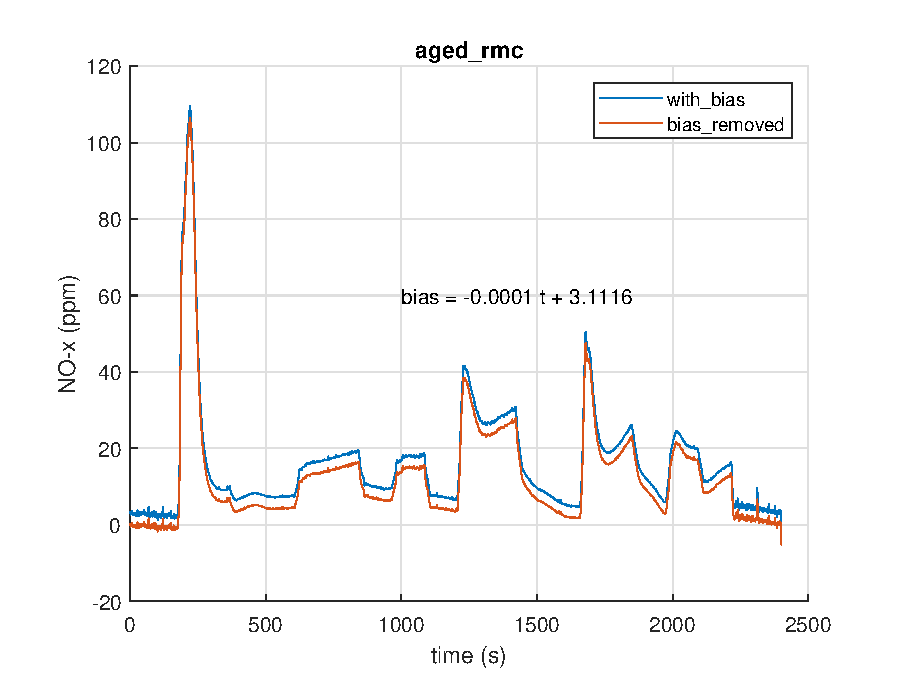
\includegraphics[width=\textwidth]{./figs/chi_est/aged_rmc_NOx_bias.eps}
        \end{figure}
    \end{minipage}
    \begin{minipage}{0.49\textwidth}
        \begin{figure}[H]
            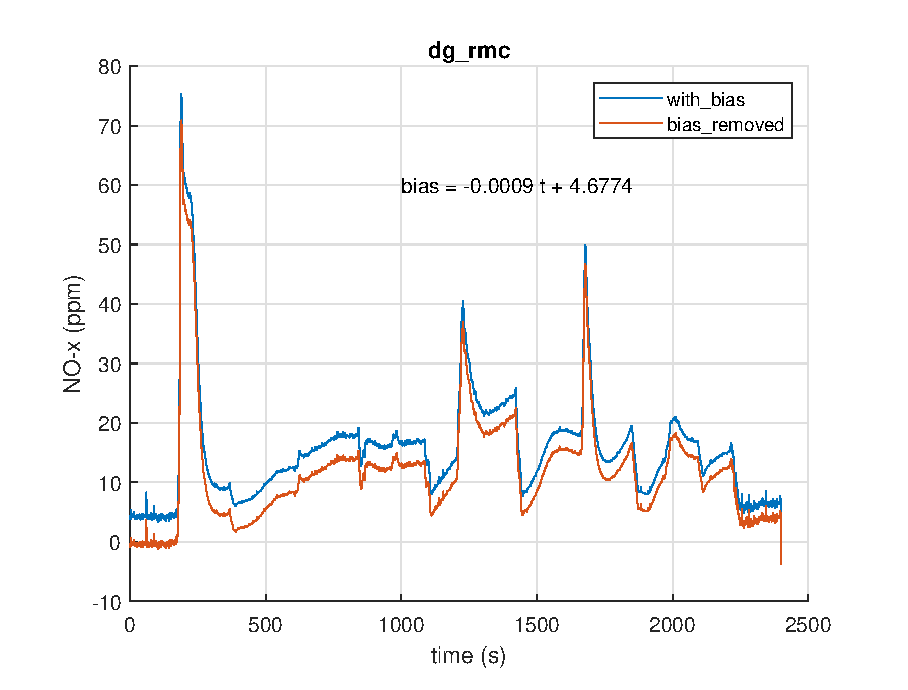
\includegraphics[width=\textwidth]{./figs/chi_est/dg_rmc_NOx_bias.eps}
        \end{figure}
    \end{minipage}
        \caption{Sensor bias correction for RMC cycles}
\end{figure}



\itbf{Effect of $NH_3$ sensor bias and minimum threshold for cross-sensitivity}\\
The ammonia sensor used for ammonia measurement also has bias and there is a
threshold on ammonia for which the $NO_x$ sensor becomes cross-sensitive to
ammonia. Thus the expression for cross-sensitivity becomes:

\begin{align*}
    y_1 &= \lr{x_1 - b_0} + \chi (x_2 - b_{th})\\
\end{align*}

\itbf{Least-squares estimation assuming temperature independence}\\
\itbf{Assumption}: The temperature changes in RMC cycle don't affect the
cross-sensitivity factor significantly. Thus, it can be treated as a constant
w.r.t temperature fluctuations in that range.

We have,
\begin{align*}
    \underbrace{y_1 - x_1}_{\pmb y} &= \underbrace{\bm{x_2 & -1}}_{\pmb \phi^T} \underbrace{\bm{ \chi \\ \underbrace{\chi b_{th} + b_0}_{=b}}}_{ \pmb \theta}\\
\end{align*}

\begin{figure}[H]
    \begin{minipage}{0.49\textwidth}
        \begin{figure}[H]
            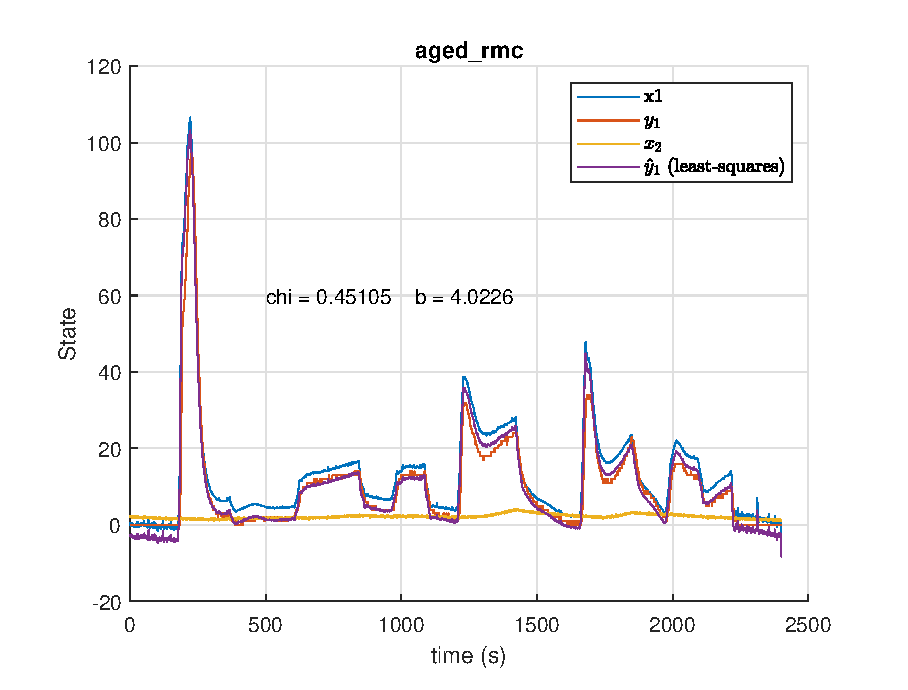
\includegraphics[width=\textwidth]{./figs/chi_est/aged_rmc_chi.eps}
        \end{figure}
    \end{minipage}
    \begin{minipage}{0.49\textwidth}
        \begin{figure}[H]
            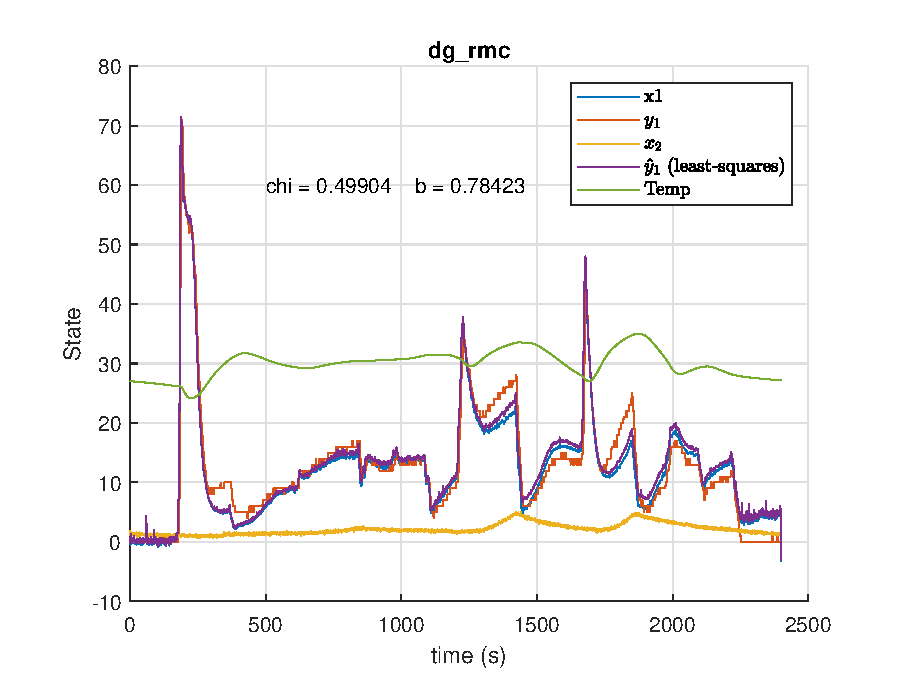
\includegraphics[width=\textwidth]{./figs/chi_est/dg_rmc_chi.eps}
        \end{figure}
    \end{minipage}
        \caption{$\chi$ estimation for RMC cycles}
\end{figure}

\begin{figure}[H]
    \centering
    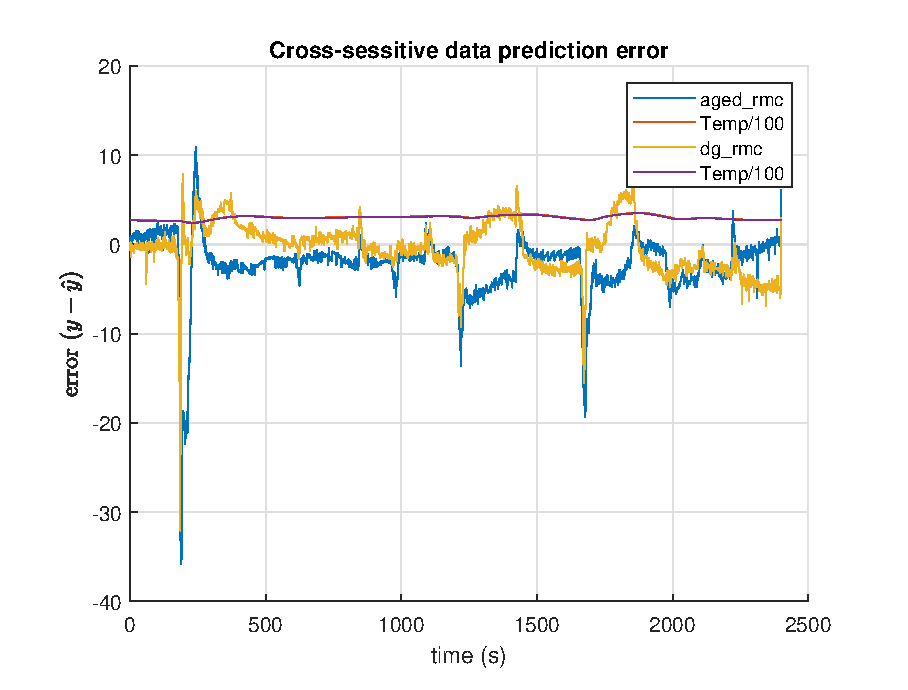
\includegraphics[width = 0.5 \textwidth]{./figs/chi_est/chi_error.eps}
    \caption{Error in $\chi$ estimation}
\end{figure}

The error can be reduced by introducing the effects of temperature into $\chi$.


\itbf{$\chi$ as a temperature function}\\
For simplicity, $\chi$ is assumed to be a linear function of temperature.
\begin{align*}
    \chi(T) &= a T - b_T
\end{align*}

\itbf{Least-squares estimation with temperature dependence}\\
Assuming the sensor-bias is not time-varying ($\because$ $b_1$ is small). The
sensor bias, cross-sensitivity threshold and temperature dependence can be
combined into:

\begin{align*}
    y_1 &=  \lr{x_1 - b_0} + \lr{aT - b_{T}} \lr{x_2 - b_{th}}\\
    \lr{y_1 - x_1} &= a T x_2 - a b_{th} T - b_{T} x_2 + (b_T b_{th} - b_0)\\
    \underbrace{y_1 - x_1}_{\pmb y} &= \underbrace{\bm{T x_2 & -T & -x_2 & 1}}_{\pmb \phi^T} \underbrace{\bm{a \\ a b_{th} \\ b_T \\ b_T b_{th} - b_0}}_{\pmb \theta}\\
\end{align*}

\begin{figure}[H]
    \begin{minipage}{0.49\textwidth}
        \begin{figure}[H]
            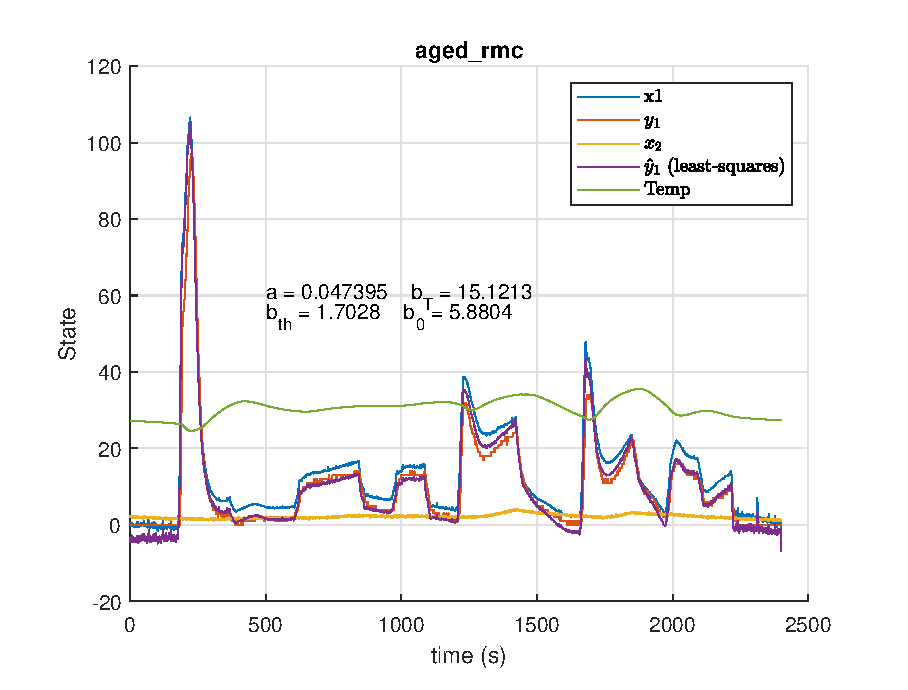
\includegraphics[width=\textwidth]{./figs/chi_est/aged_rmc_chiT.eps}
        \end{figure}
    \end{minipage}
    \begin{minipage}{0.49\textwidth}
        \begin{figure}[H]
            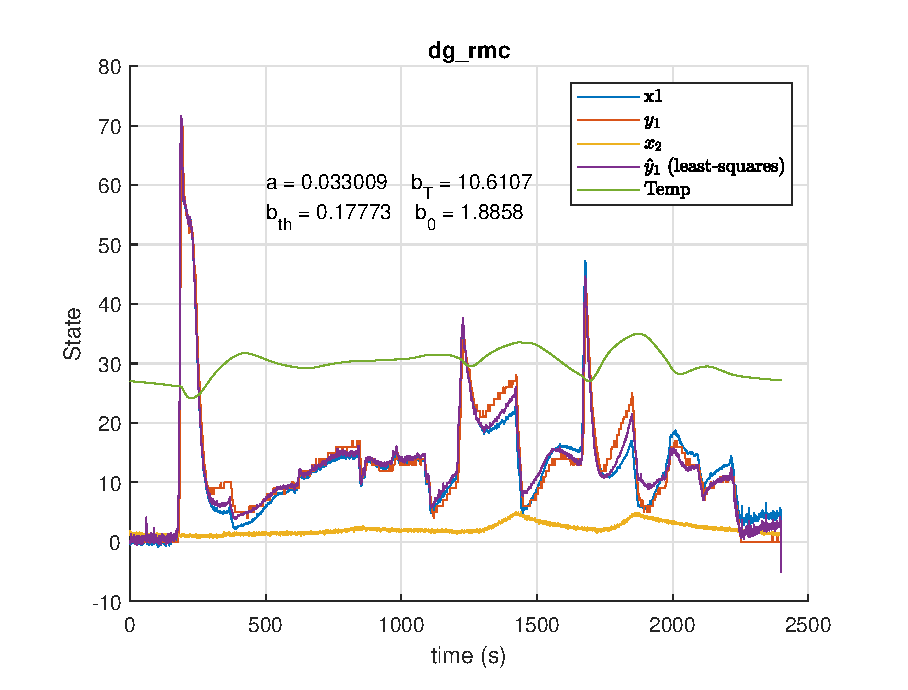
\includegraphics[width=\textwidth]{./figs/chi_est/dg_rmc_chiT.eps}
        \end{figure}
    \end{minipage}
        \caption{$\chi$ estimation for rmc cycles}
\end{figure}

\begin{figure}[H]
    \begin{minipage}{0.49\textwidth}
        \begin{figure}[H]
            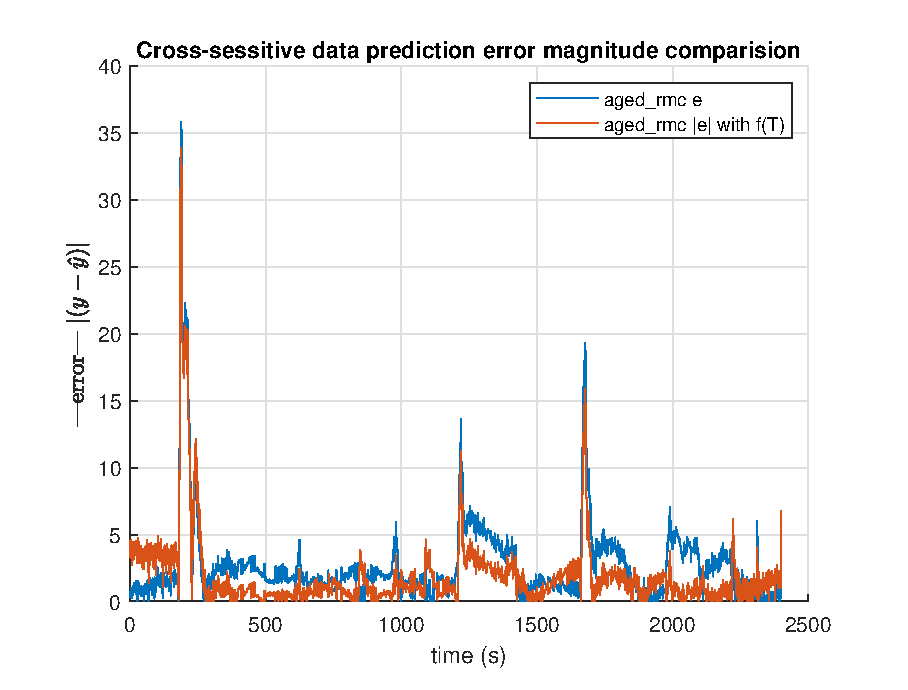
\includegraphics[width=\textwidth]{./figs/chi_est/aged_error_comp.eps}
        \end{figure}
    \end{minipage}
    \begin{minipage}{0.49\textwidth}
        \begin{figure}[H]
            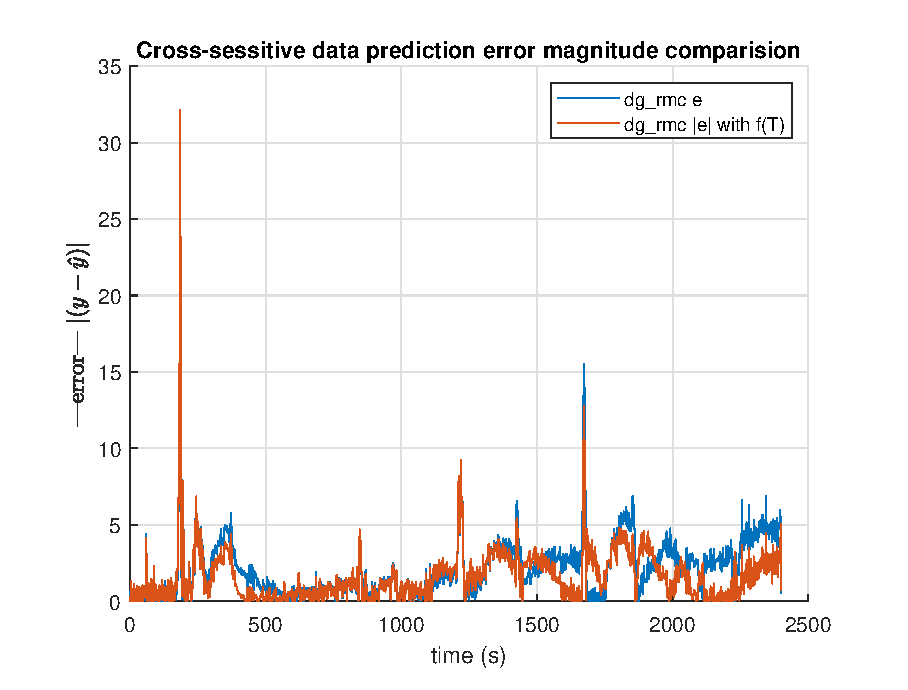
\includegraphics[width=\textwidth]{./figs/chi_est/dg_error_comp.eps}
        \end{figure}
    \end{minipage}
        \caption{Effect of temperature on prediction errors for $\chi$ estimation in RMC cycles}
\end{figure}


Introducing temperature clearly decreases the prediction error in the model. However, the reduction in error, while noticeable, is not significant when compared to the temperature-independent model, whose error remains within acceptable limits.
